\documentclass[leno,xcolor=dvipsnames]{beamer}
\usetheme[
    block=fill,         % ブロックに背景をつける
    progressbar=foot,   % 各スライドの下にプログレスバー
    numbering=fraction  % 合計ページ数を表示
]{metropolis}           % Use metropolis theme

\usepackage{luatexja}% 日本語したい
\usepackage[ipaex]{luatexja-preset}% IPAexフォントしたい
\renewcommand{\kanjifamilydefault}{\gtdefault}% 既定をゴシック体に
\makeatletter
\newcommand{\figcaption}[1]{\def\@captype{figure}\caption{#1}}
\newcommand{\tblcaption}[1]{\def\@captype{table}\caption{#1}}
\makeatother

\usepackage{float}
\usepackage{wrapfig}  % 図の回り込み
\usepackage{blindtext}
\usepackage{booktabs}
\usepackage{multirow}
\usepackage{ascmac}
\usepackage{fancybox}
\usepackage{amsmath}
\usepackage{mathtools}
\usepackage{siunitx}
\usepackage{tikz}
\usetikzlibrary {arrows.meta}
\usetikzlibrary {bending}
\usepackage{listings}
\lstset{
    frame=single,
    basicstyle=\tiny\ttfamily,
    tabsize=4
}

\title{進捗報告}
\date{\today}
\author{水野泰旭}
\institute{弘前大学理工学部電子情報工学科4年}
\subject{}
\begin{document}
  \maketitle

  \begin{frame}{目次}
    \tableofcontents
  \end{frame}

  \begin{frame}
    \section{F1スコア}
  \end{frame}

  \begin{frame}{macro-F1スコアの計算}
    混同行列を用いて計算していく。
    \begin{figure}[H]
      \centering  
      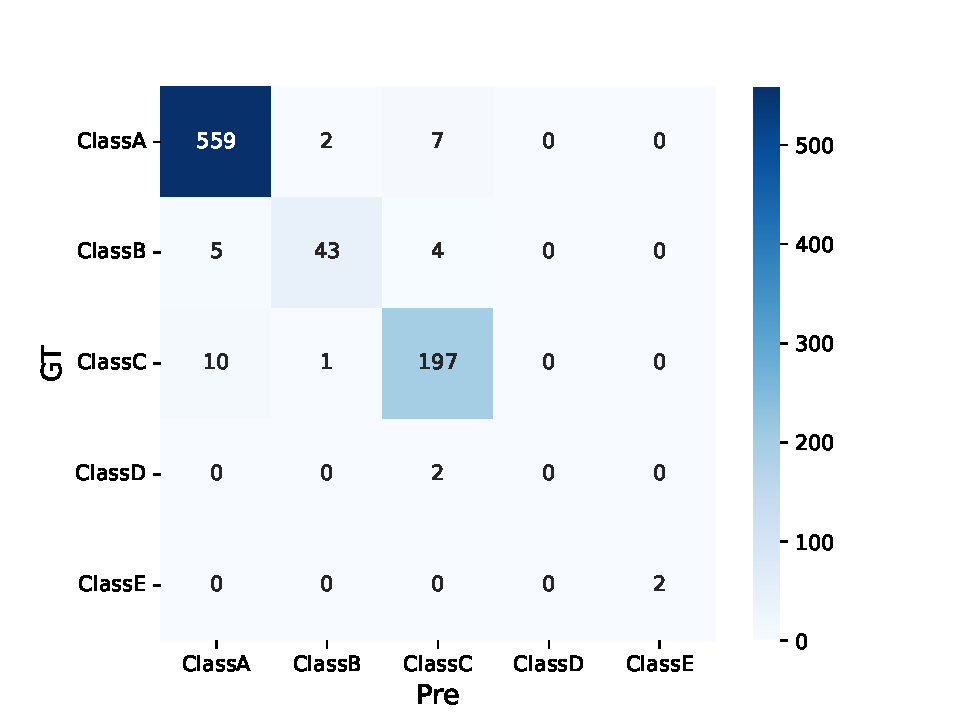
\includegraphics[keepaspectratio, scale=0.5]{images/deepimfam_confusion_matrix_cnt.pdf}
    \end{figure}
  \end{frame}

  \begin{frame}{macro-F1スコアの計算}
    \begin{figure}[h]
      \def\@captype{table}
      \begin{minipage}[t]{.48\textwidth}
        \tblcaption{ClassA} \label{tb:ClassA}
        \begin{center}
          \begin{tabular}{cccc}
            \toprule
            \multicolumn{2}{c}{} & \multicolumn{2}{c}{予測値} \\ \cline{3-4}
            & & 陽性 & 陰性 \\
            \midrule
            \multirow{2}{*}{正解率} & 陽性 & TP & FN \\
            & 陰性 & FP & TN \\
            \bottomrule
          \end{tabular}
        \end{center}
      \end{minipage}
      \hfill
      \begin{minipage}[c]{.48\textwidth}
        \centering
        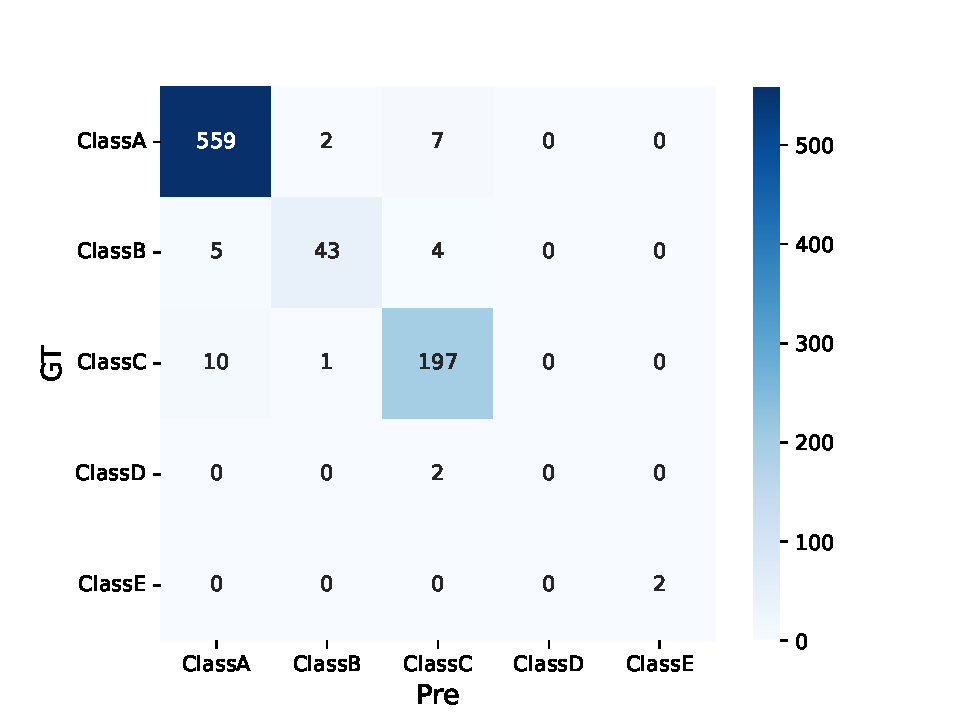
\includegraphics[keepaspectratio, scale=0.4]{images/deepimfam_confusion_matrix_cnt.pdf}
        \caption{図の見出し}
        \label{図へのラベル}
      \end{minipage}
    \end{figure}
  \end{frame}

\end{document}


